%%%%%%%%%%%%%%%%%%%%%%%%%%%%%%%%%%%%%%%%%%%%%%%%%%%%%%%%%%%%%%%%%%%%%%%%%%%%%%%%%%
% Workflow demo: email triage. Four nodes (two plain functions, two LLM calls), a richer state,
% one conditional edge. Code: Code/langgraph/workflow_demo/email_triage.py (tested with a fake model).
% Order: problem, design, then one code piece per slide, assemble, visualise, run, comparison.
\begin{frame}[fragile]\frametitle{}
\begin{center}
{\Large Workflow Demo: Email Triage}

{\tiny (A fixed path with several nodes: some plain code, some LLM calls)}
\end{center}
\end{frame}

%%%%%%%%%%%%%%%%%%%%%%%%%%%%%%%%%%%%%%%%%%%%%%%%%%%%%%%%%%%
\begin{frame}[fragile]\frametitle{The Problem: Email Triage}
      \begin{itemize}
        \item \textbf{Goal}: handle each incoming email without a person reading every one.
        \item \textbf{Steps}: read the email, decide whether it is spam, then either move it to junk or draft a reply.
        \item The steps and their order are known in advance, so this is a \textbf{workflow}, not a free-roaming agent.
        \item Two steps are plain code (split the email into words, move to junk). Two need language skills (judge spam, write a reply), so they call an LLM.
        \item One decision splits the path: spam or legitimate.
      \end{itemize}
\end{frame}

%%%%%%%%%%%%%%%%%%%%%%%%%%%%%%%%%%%%%%%%%%%%%%%%%%%%%%%%%%%
\begin{frame}[fragile]\frametitle{The Design: Four Nodes and One Decision}
\adjustbox{valign=t}{%
\begin{minipage}{0.5\linewidth}
      \begin{itemize}
        \item \textbf{State}: the email, its words, a spam flag, a draft and a log that every node adds to.
        \item \textbf{Plain nodes}: \texttt{read\_email}, \texttt{handle\_spam}.
        \item \textbf{LLM nodes} (shaded): \texttt{classify\_email}, \texttt{draft\_reply}.
        \item \textbf{Conditional edge}: after \texttt{classify\_email}, spam goes to \texttt{handle\_spam}, everything else to \texttt{draft\_reply}.
      \end{itemize}
\end{minipage}%
}%
\hfill%
\adjustbox{valign=t}{%
\begin{minipage}{0.46\linewidth}
\begin{center}
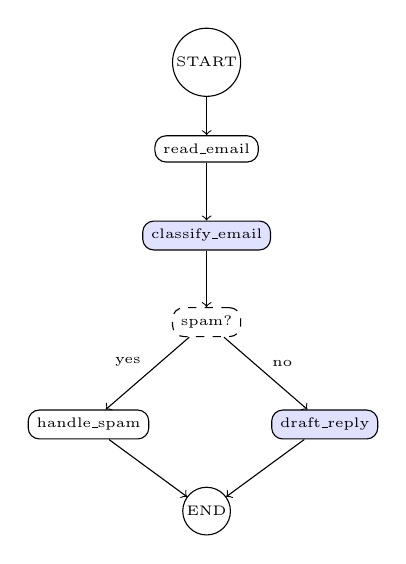
\begin{tikzpicture}
\tiny
\node[draw,circle,inner sep=1pt] (s) at (0,5.2) {START};
\node[draw,rounded corners,inner sep=3pt] (r) at (0,4.1) {read\_email};
\node[draw,rounded corners,inner sep=3pt,fill=blue!12] (c) at (0,3.0) {classify\_email};
\node[draw,dashed,rounded corners,inner sep=3pt] (q) at (0,1.9) {spam?};
\node[draw,rounded corners,inner sep=3pt] (h) at (-1.5,0.6) {handle\_spam};
\node[draw,rounded corners,inner sep=3pt,fill=blue!12] (d) at (1.5,0.6) {draft\_reply};
\node[draw,circle,inner sep=1pt] (e) at (0,-0.5) {END};
\draw[->] (s) -- (r);
\draw[->] (r) -- (c);
\draw[->] (c) -- (q);
\draw[->] (q) -- node[above left] {yes} (h);
\draw[->] (q) -- node[above right] {no} (d);
\draw[->] (h) -- (e);
\draw[->] (d) -- (e);
\end{tikzpicture}
\end{center}
\tiny{Shaded nodes call an LLM; the dashed box is the conditional edge.}
\end{minipage}%
}
\end{frame}

%%%%%%%%%%%%%%%%%%%%%%%%%%%%%%%%%%%%%%%%%%%%%%%%%%%%%%%%%%%
\begin{frame}[fragile]\frametitle{Step 1: Define the State}
      \begin{itemize}
        \item The state holds everything the workflow knows: the input, the results so far, and a log.
        \item Fields with no reducer are \textbf{overwritten} by each update (\texttt{is\_spam}, \texttt{draft}).
        \item \texttt{log} has a reducer, \texttt{operator.add}: each node \textbf{adds} its own line to the list.
      \end{itemize}
\begin{lstlisting}[language=Python]
import operator
from typing import Annotated
from pydantic import BaseModel, Field

class EmailState(BaseModel):
    email: str                              # input
    words_list: list[str] = Field(default_factory=list)   # set by read_email, read by classify_email
    is_spam: bool = False                   # set by classify_email
    draft: str = ""                         # set by draft_reply
    log: Annotated[list[str], operator.add] = Field(default_factory=list)   # audit trail
\end{lstlisting}
\end{frame}

%%%%%%%%%%%%%%%%%%%%%%%%%%%%%%%%%%%%%%%%%%%%%%%%%%%%%%%%%%%
\begin{frame}[fragile]\frametitle{Step 2: Plain-Function Nodes}
      \begin{itemize}
        \item A node is just a Python function: it reads the state and returns \textbf{only what changed}.
        \item These two use no LLM at all: ordinary code is the right tool when the rule is exact.
        \item \texttt{read\_email} splits the email into words and keeps the first 200, so the LLM prompt stays short. The next node reads that list from the state.
        \item Cheap, fast and fully predictable: the same input always gives the same output.
      \end{itemize}
\begin{lstlisting}[language=Python]
MAX_WORDS = 200

def read_email(state: EmailState):
    return {"words_list": state.email.split()[:MAX_WORDS],
            "log": ["read: email received"]}

def handle_spam(state: EmailState):
    return {"log": ["spam: moved to junk"]}
\end{lstlisting}
\end{frame}

%%%%%%%%%%%%%%%%%%%%%%%%%%%%%%%%%%%%%%%%%%%%%%%%%%%%%%%%%%%
\begin{frame}[fragile]\frametitle{Step 3: LLM Nodes}
      \begin{itemize}
        \item An LLM node is the same kind of function; inside it calls the LLM.
        \item \texttt{classify\_email}: the LLM judges the words that \texttt{read\_email} left in the state; our code turns its one-word answer into a boolean.
        \item \texttt{draft\_reply}: the LLM writes the text, which goes into the state.
        \item \texttt{startswith}, because "not spam" also contains the word "spam".
      \end{itemize}
% [code-font: forced \scriptsize | overflow at the default size]
\begin{lstlisting}[language=Python, basicstyle=\scriptsize\ttfamily]
from llm_config import get_llm
llm = get_llm()                                  # the LLM

def classify_email(state: EmailState):
    text = " ".join(state.words_list)            # the words read_email kept
    answer = llm.invoke("Classify as spam or legitimate, one word:\n" + text).content
    answer = answer.strip().lower()
    return {"is_spam": answer.startswith("spam"), "log": [f"classify: {answer}"]}

def draft_reply(state: EmailState):
    reply = llm.invoke("Draft a short, professional reply:\n" + state.email).content
    return {"draft": reply, "log": ["draft: reply written"]}
\end{lstlisting}
\end{frame}

%%%%%%%%%%%%%%%%%%%%%%%%%%%%%%%%%%%%%%%%%%%%%%%%%%%%%%%%%%%
\begin{frame}[fragile]\frametitle{Step 4: The Router (Conditional Edge)}
      \begin{itemize}
        \item The router reads the state and returns a label; it does not change the state.
        \item Here the decision is made by code, from the flag the LLM node wrote.
        \item The label is mapped to the next node when the graph is assembled.
      \end{itemize}
\begin{lstlisting}[language=Python]
def route_email(state: EmailState):
    return "spam" if state.is_spam else "legit"
\end{lstlisting}
\end{frame}

%%%%%%%%%%%%%%%%%%%%%%%%%%%%%%%%%%%%%%%%%%%%%%%%%%%%%%%%%%%
\begin{frame}[fragile]\frametitle{Step 5: Assemble the Graph}
      \begin{itemize}
        \item Register every node by name, then the edges: normal edges, then the one conditional edge.
        \item Both branches end at END.
      \end{itemize}
\begin{lstlisting}[language=Python]
from langgraph.graph import StateGraph, START, END

workflow = StateGraph(EmailState)
workflow.add_node("read_email", read_email)
workflow.add_node("classify_email", classify_email)
workflow.add_node("handle_spam", handle_spam)
workflow.add_node("draft_reply", draft_reply)

workflow.add_edge(START, "read_email")
workflow.add_edge("read_email", "classify_email")
workflow.add_conditional_edges(
    "classify_email", route_email,
    {"spam": "handle_spam", "legit": "draft_reply"})   # label -> next node
workflow.add_edge("handle_spam", END)
workflow.add_edge("draft_reply", END)

graph = workflow.compile()
\end{lstlisting}
\end{frame}

%%%%%%%%%%%%%%%%%%%%%%%%%%%%%%%%%%%%%%%%%%%%%%%%%%%%%%%%%%%
\begin{frame}[fragile]\frametitle{Visualise the Compiled Graph}
\adjustbox{valign=t}{%
\begin{minipage}{0.5\linewidth}
      \begin{itemize}
        \item Draw the graph and compare it with the design.
        \item Dashed arrows are the conditional edge, labelled with the router's return values.
        \item \texttt{draw\_mermaid()} prints the same graph as text, offline; in a notebook, \texttt{draw\_mermaid\_png()} shows it as a picture.
      \end{itemize}
% [upgrade-deck: moved 2026-10-19 | Task 1b | the listing now follows both columns so it is the last element of the frame]
\end{minipage}%
}%
\hfill%
\adjustbox{valign=t}{%
\begin{minipage}{0.46\linewidth}
\begin{center}
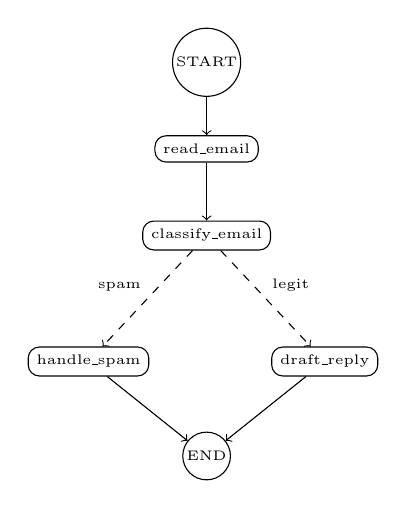
\begin{tikzpicture}
\tiny
\node[draw,circle,inner sep=1pt] (s) at (0,5.2) {START};
\node[draw,rounded corners,inner sep=3pt] (r) at (0,4.1) {read\_email};
\node[draw,rounded corners,inner sep=3pt] (c) at (0,3.0) {classify\_email};
\node[draw,rounded corners,inner sep=3pt] (h) at (-1.5,1.4) {handle\_spam};
\node[draw,rounded corners,inner sep=3pt] (d) at (1.5,1.4) {draft\_reply};
\node[draw,circle,inner sep=1pt] (e) at (0,0.2) {END};
\draw[->] (s) -- (r);
\draw[->] (r) -- (c);
\draw[->,dashed] (c) -- node[above left] {spam} (h);
\draw[->,dashed] (c) -- node[above right] {legit} (d);
\draw[->] (h) -- (e);
\draw[->] (d) -- (e);
\end{tikzpicture}
\end{center}
\tiny{Output of the compiled graph (redrawn).}
\end{minipage}%
}

\begin{lstlisting}[language=Python]
g = graph.get_graph()
print(g.draw_mermaid())
\end{lstlisting}
\end{frame}

%%%%%%%%%%%%%%%%%%%%%%%%%%%%%%%%%%%%%%%%%%%%%%%%%%%%%%%%%%%
\begin{frame}[fragile]\frametitle{Run It and Watch Each Node}
      \begin{itemize}
        \item \texttt{stream\_mode="updates"} shows, for every node, only what it returned.
        \item The spam path stops after \texttt{handle\_spam}: there is no second LLM call.
        \item Output of a real run with \texttt{gemma-2-2b-it} in LM Studio; the wording of a draft varies.
      \end{itemize}
\begin{lstlisting}[language=Python]
email = "URGENT! You have won 1,000,000 dollars. Click here now!!!"
for update in graph.stream(EmailState(email=email), stream_mode="updates"):
    print(update)

# {'read_email':     {'words_list': ['URGENT!', 'You', 'have', ...], 'log': ['read: email received']}}
# {'classify_email': {'is_spam': True, 'log': ['classify: spam']}}
# {'handle_spam':    {'log': ['spam: moved to junk']}}
#
# A legitimate email takes the other branch:
# {'classify_email': {'is_spam': False, 'log': ['classify: legitimate']}}
# {'draft_reply':    {'draft': 'Subject: Re: Project Timeline ... Yes, I would be happy to meet ...', ...}}
\end{lstlisting}
\end{frame}

%%%%%%%%%%%%%%%%%%%%%%%%%%%%%%%%%%%%%%%%%%%%%%%%%%%%%%%%%%%
\begin{frame}[fragile]\frametitle{Workflow versus Agent: Same Pieces, Different Control}
      \begin{itemize}
        \item \textbf{Same pieces}: a state, nodes that are plain functions, normal and conditional edges.
        \item \textbf{This workflow}: the developer fixed the path; the LLM works \emph{inside} two of the steps. Predictable, cheap and easy to test.
        % [upgrade-deck: commented out 2026-10-19 | Task 5c | two sentences split into a lead plus one sub-point]
        % \item \textbf{An agent}: the LLM decides at run time whether to call a tool, and the graph loops back until it is done. Add a loop-back edge and a tools node to get one.
        \item \textbf{An agent}: the LLM decides at run time whether to call a tool, and the graph loops back until it is done.
        \begin{itemize}
          \item To get one, add a tools node and a loop-back edge.
        \end{itemize}
        \item In both, a node can hold any code: an LLM call, an API call, plain logic, or a whole agent.
        \item Choose the least freedom that does the job.
      \end{itemize}
\end{frame}

%%%%%%%%%%%%%%%%%%%%%%%%%%%%%%%%%%%%%%%%%%%%%%%%%%%%%%%%%%%
\begin{frame}[fragile]\frametitle{Beyond the Basics: More Features}
      \begin{itemize}
        % [upgrade-deck: commented out 2026-10-19 | Task 5c | long bullet split into a lead plus one sub-point]
        % \item \textbf{Human in the loop}: \texttt{interrupt()} pauses a node and waits; \texttt{Command(resume=...)} continues. Use it for approval before a payment, a send or a delete, or for editing a draft.
        \item \textbf{Human in the loop}: \texttt{interrupt()} pauses a node and waits; \texttt{Command(resume=...)} continues.
        \begin{itemize}
          \item Use it for approval before a payment, a send or a delete, or for editing a draft.
        \end{itemize}
        \item \textbf{Checkpointing and memory}: a checkpointer saves the state after each step; a \texttt{thread\_id} picks the conversation. It enables pause and resume, follow-up questions and replay.
        \item \textbf{Streaming}: watch progress instead of waiting for the end.
        \item \textbf{Command and Send}: one return value can update state and choose the next node; \texttt{Send} fans out the same node over many items in parallel.
        \item \textbf{Subgraphs and multi-agent}: a node can itself be a graph, so agents can be composed.
        \item Each of these is added to the same graph; the nodes and edges you wrote stay as they are.
      \end{itemize}
\end{frame}

%%%%%%%%%%%%%%%%%%%%%%%%%%%%%%%%%%%%%%%%%%%%%%%%%%%%%%%%%%%
\begin{frame}[fragile]\frametitle{Streaming and Human Approval in a Few Lines}
      \begin{itemize}
        \item \textbf{Stream modes}: \texttt{values} (full state after each step), \texttt{updates} (only what each node changed), \texttt{messages} (LLM tokens as they arrive), \texttt{custom} (your own progress events).
        \item \textbf{Approval}: the graph needs a checkpointer and a \texttt{thread\_id}, so it can stop and come back. Here a person approves the draft before it is sent.
      \end{itemize}
% [code-font: forced \scriptsize | overflow at the default size]
\begin{lstlisting}[language=Python, basicstyle=\scriptsize\ttfamily]
for chunk in graph.stream(EmailState(email=email), stream_mode="updates"):
    print(chunk)                                  # {node_name: what it returned}

from langgraph.types import interrupt, Command
from langgraph.checkpoint.memory import InMemorySaver

def approve_reply(state):                         # a node after draft_reply that waits for a person
    ok = interrupt({"question": "Send this reply?", "draft": state.draft})
    return {"log": [f"approval: {ok}"]}

graph = workflow.compile(checkpointer=InMemorySaver())
cfg = {"configurable": {"thread_id": "t1"}}
graph.invoke(EmailState(email=email), cfg)        # runs until interrupt(), then pauses
graph.invoke(Command(resume=True), cfg)           # resumes; ok == True
\end{lstlisting}
\end{frame}

%%%%%%%%%%%%%%%%%%%%%%%%%%%%%%%%%%%%%%%%%%%%%%%%%%%%%%%%%%%
\begin{frame}[fragile]\frametitle{Demo Summary}
      \begin{itemize}
        \item \textbf{Problem}: handle each email without a person reading every one.
        \item \textbf{Design}: four nodes (two plain code, two LLM), one conditional edge, two paths to END.
        \item \textbf{State}: the email, \texttt{words\_list}, \texttt{is\_spam}, \texttt{draft} and a \texttt{log} with a reducer.
        \item \textbf{Run}: each streamed update shows what one node returned; the spam path makes only one LLM call.
        \item \textbf{Remember}: a node is any Python function, an edge is normal or conditional, the state is the shared context, and the LLM is swappable through one config.
      \end{itemize}
\end{frame}

%%%%%%%%%%%%%%%%%%%%%%%%%%%%%%%%%%%%%%%%%%%%%%%%%%%%%%%%%%%
\begin{frame}[fragile]\frametitle{Quick Check: The Email Workflow}
\begin{block}{Think About It}
A spam email goes through this graph. How many LLM calls are made, and why?
\begin{enumerate}
  \item[A.] Two: every node calls the LLM
  \item[B.] One: only \texttt{classify\_email}; the router and \texttt{handle\_spam} are plain code
  \item[C.] One: the router asks the LLM which branch to take
  \item[D.] Zero: the words in \texttt{words\_list} already say it is spam
\end{enumerate}
\end{block}
\end{frame}

%%%%%%%%%%%%%%%%%%%%%%%%%%%%%%%%%%%%%%%%%%%%%%%%%%%%%%%%%%%
\begin{frame}[fragile]\frametitle{Quick Check: The Email Workflow}
\begin{block}{Answer}
\textbf{Correct: B.} Only \texttt{classify\_email} calls the LLM. \texttt{route\_email} just reads the \texttt{is\_spam} flag that node wrote, and \texttt{handle\_spam} is plain code, so \texttt{draft\_reply} (the second LLM call) is never reached. Option C is wrong because the router is code, and D is wrong because nothing in \texttt{read\_email} judges the content.
\end{block}
\end{frame}
